\section{Pauli Formalism}
In the following we will develop a convenient formalism build from the three Pauli symbols ${\sigma_0,\sigma_1,\sigma_2,\sigma_3}$ that is sufficient to represent all operations on quantum computers. 
The primitive symbols ${\sigma_1,\sigma_2,\sigma_3}$ have a representation as $2\times 2$ Pauli matrices, while $\sigma_0$ is just the unit operation.
\begin{def*}[Pauli Matrix]
\begin{align}
        \sigma_1\equiv X = \begin{pmatrix}
        0 & 1 \\ 1 & 0
    \end{pmatrix}, \;\;        \sigma_2\equiv Y = \begin{pmatrix}
        0 & -i \\ i & 0
    \end{pmatrix},\;\;        \sigma_3\equiv Z=  \begin{pmatrix}
        1 & 0 \\ 0 & -1
    \end{pmatrix}
\end{align}
\end{def*}
Besides many other properties, the Pauli matrices are \textit{unitary} and \textit{Hermitian} (and therefore also \textit{self-inverse})~\footnote{they are also traceless, but we won't need this property here. Note that this is the reason why $\sigma_0 = 1_{2\times 2}$ is formally not a Pauli matrix. We will however be sloppy with the naming.}
\begin{theorem*}[pauli algebra]
Pauli matrices are unitary and Hermitian at the same time
\begin{align}
    \sigma_k ^\dagger = \sigma_k = \sigma_k^{-1}.\label{eq:pauli-algebra}
\end{align}
The product of two distinct Pauli matrices (not considering the unit matrix) will be proportional to the corresponding third Pauli matrix 
\begin{align}
    &XY = iZ, \;\; YX = -iZ\\
    &ZX = iY, \;\; XZ = -iY\\
    &YZ = iX, \;\; ZY = -iX
\end{align}
where the sign can be determined if the string of Paulis from left to right is an odd or even permutation from $XYZ$.
From the multiplication it follows direclty that the Pauli matrices transform anti-symmeric under themselves
\begin{align}
    \sigma_k \sigma_l \sigma_k = - \sigma_l,\; \forall k\neq l\in \left\{x,y,z\right\}.
\end{align}
\end{theorem*}
Take as explicit example (which we will also need further down)
\begin{align}
    XZX = -Z\label{eq:XZX=-Z}.
\end{align}
We can now generate operations on multiple qubits via tensor products.
\begin{def*}[Paulistring]
An $N$-qubit Paulistring is given by
    \begin{align}
        P_{\mathbf{k}} = \bigotimes_{i=1} ^{N} \sigma_{k_i}
    \end{align}
    where $\mathbf{k}=\left[k_1,k_2,k_3,\dots, k_N\right]$ and each $k_i\in \left\{0,1,2,3\right\}$
\end{def*}
It is often useful to use ``normal'' products instead of tensor products and write the qubit onto which the Pauli matrix acts in parenthesis
The two notations below are then equivalent
    \begin{align}
        P_{\mathbf{k}} = \bigotimes_{i=1} ^{N} \sigma_{k_i}=\prod_{i=1} ^{N} \sigma_{k_i}(i)
    \end{align}
and the latter has the advantage that we can drop unit matrices. Some examples
\begin{align}
    &1\otimes X \otimes Y = Y(1)X(2) \\
    &\sigma_x \otimes 1 \otimes \sigma_z = Z(1)X(3).
\end{align}
As the Pauli matrices, any Paulistring is \textit{unitary} and \textit{Hermitian}
\begin{align}
    P_\mathbf{k} ^\dagger = P_\mathbf{k} = P_\mathbf{k}^{-1}.
\end{align}

\begin{theorem*}[Pauli basis]
Any $2\times 2$ matrix can be represented as a linear combination of the four Pauli symbols.
\end{theorem*}
We can see this by representing the ``standard'' basis in terms of the Paulis
\begin{align}
    &\begin{pmatrix}
        1 & 0 \\0 & 0
    \end{pmatrix} = \ket{0}\bra{0}=  \frac{1}{2}\left(1 + Z\right),\;\;
    \begin{pmatrix}
    0 & 0 \\0 & 1
    \end{pmatrix} = \frac{1}{2}\left(1 - Z\right) = \ket{1}\bra{1}\\
    &\begin{pmatrix}
        0 & 1 \\0 & 0
    \end{pmatrix} = \ket{0}\bra{1} =  \frac{1}{2}\left(X + iY\right),\;\;    \begin{pmatrix}
        0 & 0 \\1 & 0
    \end{pmatrix}  = \ket{1}\bra{0}= \frac{1}{2}\left(X - iY\right) 
\end{align}
where the short-notation $\sigma_{\pm} = 1/2(X \pm iY)$ is fairly common.
In the same manner we have
\begin{theorem*}[Pauli basis]
Any $2^N\times 2^N$ matrix can be represented as a linear combination of all possible $N$-qubit Pauli strings.
\end{theorem*}
You can see this by thinking about the standard basis in $2^N$ dimension as the tensor product of the standard basis in $2^{N-1}$ dimensions. Just try to build the 4 basis matrices for $4\times 4$ matrices as tensor products from the $2\times 2$ standard basis matrices. Now you can use the formulas above to decompose back into Paulistrings. Here is an example
\begin{align}
    \begin{pmatrix}
        0 & 0 & 0 & 0\\
0 & 0 & 1 & 0\\
0 & 0 & 0 & 0\\
0 & 0 & 0 & 0\\
    \end{pmatrix} &= \ket{1}\bra{2} = \ket{01}\bra{10}\nonumber\\ 
    &=\ket{0}\bra{1}\otimes\ket{1}\bra{0} = \sigma_+ \otimes \sigma_- \nonumber\\
    &= \frac{1}{4}\left(X\otimes X - iX\otimes Y + i Y\otimes X + Y\otimes Y\right)
\end{align}
Representing a matrix as a linear combination of Pauli matrices has some advantages compared to the standard basis.
\begin{theorem*}
    A matrix $M$ that can be represented as a linear combination of Pauli matrices
    \begin{align*}
        M = \sum_{k} c_k P_\mathbf{k}
    \end{align*}
    is Hermitian ($M^\dagger=M)$ iff all $c_k$ are real numbers, and anti-Hermitian ($M^\dagger = - M$) iff all $c_k$ are purely imaginary.
\end{theorem*}
In a way you can think about Hermitian and anti-Hermitian matrices as the equivalent of real and imaginary parts of a matrix~\footnote{You can also write any general matrix as $M=H + A$ with Hermitian $H=\frac{1}{2}(M+M^\dagger)$ and anti-Hermitian $\frac{1}{2}(M - M^\dagger)$ similar to real and imaginary parts of a complex number. In the Paulistring representation $M=\sum_k c_k P_k$ with complex numbers $c_k = a_k + ib_k$ we have $H=\sum_k a_k P_k$ and $A=\sum_k ib_k P_k$.} Just don't get confused: A Hermitian matrix can have complex entries (see for example the Pauli $Y$ matrix) but in the Pauli representation it will only have real coefficients.\\
We can use this to define a datatype with corresponding datastructure
\begin{def*}[$N$-Qubit Hermitian Operation]\phantom{...}\\
    A set of tuples $\left\{(c_k,P_\mathbf{k})\right\}_{k=1}^N$ with $c_k\in \mathbb{R} $ and $P_k$ a Paulistring.\\

    Represents the operation
    \begin{align*}
        H = \sum_k c_k P_\mathbf{k}.
    \end{align*}
\end{def*}

\subsection{Pauli Gates}

We know now how to represent any matrix on $N$-qubits, including the for important Hermitian matrices, as a linear combination of Paulistrings.
Of course we can also represent unitary matrices as linear combination of Pauli strings, compared to the Hermitian matrices there is however no simple trick on how to ensure that the matrix is unitary. 
Rather than having a sum, it is more convenient to use products to represent unitary matrices~\footnote{Hermitians are closed under addition: if $B,D$ are Hermitian then $A = B + C$ is Hermitian while unitaries are closed under multiplication: if $B,D$ are unitary, then $A = BD$ is untary.}
If we represent a unitary $U$ as a product of other unitaries $U=U_mU_{m-1}U_{m-2}\dots U_1$ we call this a quantum circuit and the individual $U_m$ quantum gates.
The Paulistrings themselves are not the best primitives for a product representation, since a product of two Paulistrings is always another Paulistring, so we would be way to restricted to represent arbitrary unitary matrices. 
\begin{def*}[Pauli Gate]
    The Pauli gate is a unitary matrix generated by a Paulistring
    \begin{align}
        R_\mathbf{k}(\theta) = e^{-i\frac{\theta}{2} P_\mathbf{k}}
    \end{align}
    where $\theta \in \mathbf{R}$ and the $-1/2$ is a convention that we will follow for consistency with the literature.
\end{def*}
It turns out that the Pauli gate is \textit{universal}, meaning roughly that we can represent any unitary as a product of Pauli gates $R_\mathbf{k}(\theta_k)$ (with corresponding angles $\theta_k$ set to concrete values) to arbitrary accuracy (so not necessarily exact, but with controllable error).  
The meaning of this statement will become clear in the next sections.
Before we turn our attention to compiling strategies with Pauli gates as gate-sets, we will take a look at common used forms and useful properties. 
\begin{theorem*}[Pauli Gate: Closed form]
All Pauli gates can be represented as
\begin{align}
    R_\mathbf{k}(\theta) = \cos\left(\frac{\theta}{2}\right) -i \sin\left(\frac{\theta}{2}\right)P_\mathbf{k}
\end{align}
\end{theorem*}
To proof the property: check the series representation for $\exp$, $\sin$, $\cos$ and use the fact that the Paulistrings are self-inverse $P_\mathbf{k}^2=1$.
From the closed form representation another useful property follows directly.
\begin{theorem*}
Paulistrings generate themselves (up to a global phase)
\begin{align}
    P_\mathbf{k} = -i R_\mathbf{k}(\pi)
\end{align}
\end{theorem*}
At this point, it might be useful to visit the appendix~\ref{sec:qubit-rep} and re-iterate what global phases are.\\

The single qubit Pauli gates (generated by $X,Y,Z$)~\footnote{the ``gate'' generated by $1$ would just be a global phase gate, and therefore not realizable in the physical sense.} are in some sense special, as they are usually considered ``standard'' operation that any high-level language should be able to support.
\begin{def*}[Single-Qubit Rotations]
    The Pauli gates generated by $X,Y,Z$ are called qubit rotations. Their matrix form (following directly from the closed-form of Pauli gates) are
    \begin{align}
        R_x(\theta) = \begin{pmatrix}
            \cos\left(\frac{\theta}{2}\right) & -i\sin\left(\frac{\theta}{2}\right) \\ -i\sin\left(\frac{\theta}{2}\right) & \cos\left(\frac{\theta}{2}\right)
        \end{pmatrix}
    \end{align}
    \begin{align}
        R_y(\theta) = \begin{pmatrix}
            \cos\left(\frac{\theta}{2}\right) & -\sin\left(\frac{\theta}{2}\right) \\ \sin\left(\frac{\theta}{2}\right) & \cos\left(\frac{\theta}{2}\right)
        \end{pmatrix}
    \end{align}
    \begin{align}
        R_z(\theta) = \begin{pmatrix}
            e^{-i\frac{\theta}{2}} & 0 \\ 0 & e^{i\frac{\theta}{2}}
        \end{pmatrix}
    \end{align}
\end{def*}
The qubit rotations are the rotation matrices for $\mathbb
{C}^2$.~\footnote{easy to see with $R_y$ which is the rotation matrix for $\mathbb{R}^2$. Just apply the matrix to any vector and see what happens.}
The fancy term here is $\operatorname{SU}(2)$, the group of ``special unitary matrices in 2 dimensions''~\footnote{special, because the determinant is always 1. We don't need the other matrices, that would then form the group $\operatorname{U}(2)$, due to the global phase equivalency. If the determinant of a matrix $U \in \mathbb{C}^{n \times n}$ is 1, then the determinant of $\tilde{U} = e^{i\varphi} U$ is $e^{i n \varphi}$. Sometimes the global phase $e^{i\varphi}$ is called a $\operatorname{U}(1)$ transformation (as you can view  it as a one dimensional matrix). So the global phase equivalence is sometimes referred to as $\operatorname{U}(1)$ invariance. }\\

\subsection{Pauli Gate Compiling}
In the following we will derive the general formula to compile an arbitrary Pauli gate $R_\mathbf{k}$ into a sequence of gates consisting only of gates in the set $\left\{\textsc{CNOT}, R_x,R_y,R_z\right\}$.\\

Lets consider the case, when all Pauli-matrices in the Paulistring $P_\mathbf{k}$ are $Z$ or $1$ -- we denote such Pauli strings as $P_\mathbf{d}$, using $\mathbf{d}$ for the index set (as it only needs to carry the non-trivial indices where the $Z$ operations act)
\begin{align}
    P_\mathbf{d}= \prod_{k\in \mathbf{d}} Z(k).
\end{align}
In this case, all standard basis states are eigenstates of $P_\mathbf{d}$~\footnote{$P_\mathbf{d}$ is a diagonal matrix, and so is $e^{-i\frac{\theta}{2}P_\mathbf{d}}$.} with eigenvalue $\pm 1$, so the gate $U_p(\theta)$ is introducing phases $e^{\mp i \frac{\theta}{2}}$ depending on the basis state it acts on. The eigenvalue is determined on the qubits where $P_\mathbf{d}$ is non-trivial -- the qubits $k\in \mathbf{d}$. If an odd number of those qubits is in state $\ket{1}$ the eigenvalue is $-1$ otherwise it is $+1$. Consider some standard computational basis state $\ket{l} \equiv \ket{l_0\dots l_{N-1}}$ on $N$ qubits
\begin{align}
    P_\mathbf{d} \ket{l_0l_1\dots l_{N-1}} =  \prod_{k\in \mathbf{d}}(-1)^{l_k} \ket{l_0l_1\dots l_{N-1}}.
\end{align}
In the same way the gate $R_{\mathbf{d}}(\theta) = e^{-i\frac{\theta}{2}P_\mathbf{d}}$ will act as
\begin{align}
    R_{P_\mathbf{d}}(\theta) \ket{l_0\dots l_{N-1}} = e^{-i\frac{\theta}{2} \prod_{k\in \mathbf{d}}{}\left(-1\right)^{l_k}} \ket{l_0\dots l_{N-1}}
\end{align}
which will evaluate to either $e^{\mp i\frac{\theta}{2}}\ket{l_0\dots l_{N-1}}$.\\


The goal is now to decompose the gate $R_{P_z}(\theta) = e^{-i\frac{\theta}{2}P_z}$ into \textsc{cnot} and single-qubit rotation gates.
At this point, we will take advantage of the property $XZX = -Z$ (see Eq.~\eqref{eq:XZX=-Z} ) of Pauli matrices 
and use \textsc{cnot} operations to flip the phase on a single $R_z$ operation placed at a qubit of our choice.
The decomposition strategy is as follows:
\begin{algo*}[$R_\mathbf{d}$ Compiling]\phantom{...}\\
Task: compile a diagonal Pauli gate $R_\mathbf{d}$ into $\textsc{cnot}$ and single Pauli rotations:\\
\begin{enumerate}
    \item pick one $k\in \mathbf{d}$
    \item add a $\textsc{cnot}(l,k)\; \forall l \in \mathbf{d}$ with $ l\neq k$
    \item place a $R_z$ rotation on qubit $k$
    \item uncompute the effect of the \textsc{cnot} sequence by adding the same sequence again.
\end{enumerate}
\end{algo*}
Let's see an example on three qubits labelled by 0,2,4 and where we pick $k=4$ in the algorithm above
\begin{equation}
    \tikzset{
        roundmini/.style={draw, circle, fill=unia2, text=white, inner sep=0.5pt, minimum size=1.2em, font=\small}
    }
    \begin{quantikz}
        \lstick{0} & \gate[style=roundmini]{\textcolor{white}{Z}} \vqw{1} & \qw \\
        \lstick{2} & \gate[style=roundmini]{\textcolor{white}{Z}} \vqw{1} & \qw \\
        \lstick{4} & \gate[style=roundmini]{\textcolor{white}{Z}}         & \qw 
    \end{quantikz}
    =
    \begin{quantikz}
        \lstick{0} & \ctrl{2} & \qw      & \qw                       & \qw      & \ctrl{2} & \qw \\
        \lstick{2} & \qw      & \ctrl{1} & \qw                       & \ctrl{1} & \qw      & \qw \\
        \lstick{4} & \targ{} & \targ{} & \gate[style=roundmini]{\textcolor{white}{Z}} & \targ{} & \targ{} & \qw 
    \end{quantikz}
\end{equation}
% \begin{align}
%     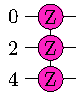
\includegraphics[height=0.1\textheight]{src/pauli_zgate_level_0.pdf}
%     \raisebox{1cm}{=}
%     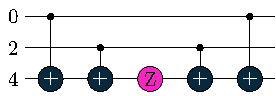
\includegraphics[height=0.1\textheight]{src/alt_pauli_zgate_level_1.pdf}.
% \end{align}
where the gates that carry the parameter $\theta$ are marked in purple.
The strategy works as well with a ``ladder'' arrangement of the \textsc{cnots}.
Take for example
\begin{equation}
    \tikzset{
        roundmini/.style={draw, circle, fill=unia2, text=white, inner sep=0.1pt, minimum size=1.2em, font=\small}
    }
    \begin{quantikz}
        \lstick{} & \gate[style=roundmini]{\textcolor{white}{Z}} \vqw{1} & \qw \\
        \lstick{} & \gate[style=roundmini]{\textcolor{white}{Z}} \vqw{1} & \qw \\
        \lstick{} & \gate[style=roundmini]{\textcolor{white}{Z}}         & \qw 
    \end{quantikz}
    =
    \begin{quantikz}
        \lstick{} & \ctrl{1} & \qw      & \qw                       & \qw      & \ctrl{1} & \qw \\
        \lstick{} & \targ{}     & \ctrl{1} & \qw                       & \ctrl{1} & \targ{}       & \qw \\
        \lstick{} & \qw & \targ{} & \gate[style=roundmini]{\textcolor{white}{Z}} & \targ{} & \qw & \qw 
    \end{quantikz}.
\end{equation}
% \begin{align}
%     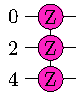
\includegraphics[height=0.1\textheight]{src/pauli_zgate_level_0.pdf}
%     \raisebox{1cm}{=}
%     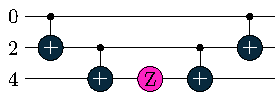
\includegraphics[height=0.1\textheight]{src/pauli_zgate_level_1.pdf}.
% \end{align}


Finally it is just a small step from the ``all-Z'' (or a  $R_\mathbf{k}$) generator to a general Pauli gate $R_\mathbf{k}$.
We essentially just have to come up with a small circuit that diagonalized $R_\mathbf{k}$ which is the same circuit that diagonalized the Pauli string $P_\mathbf{k}$ itself -- but let's clarify this first.
Assume you have a unitary that diagonalized $P_\mathbf{k}$, let's call it $U_\mathbf{k}$ since it will obviously depend on $\mathbf{k}$
\begin{align}
    U_\mathbf{k} P_\mathbf{k}U_\mathbf{k}^\dagger = P_\mathbf{d}
\end{align}
then this unitary also diagonalized $R_\mathbf{k}$ which can can easily see over the closed-form of the gate~\footnote{this relation however also holds if no closed form is available, just via the exponential series and the following trick (here shown for exponent 3): $P_\mathbf{k}^3 = P_\mathbf{k}P_\mathbf{k}P_\mathbf{k} = P_\mathbf{k}1P_\mathbf{k}1P_\mathbf{k} = P_\mathbf{k}U_\mathbf{k}^\dagger U_\mathbf{k} P_\mathbf{k}U_\mathbf{k}^\dagger U_\mathbf{k}P_\mathbf{k} $.}
\begin{align}
    U_\mathbf{k}R_\mathbf{k}(\theta)U_\mathbf{k}^\dagger &= \cos(\theta/2) -i \sin(\theta_2)U_\mathbf{k}P_\mathbf{k}U_\mathbf{k}^\dagger  \nonumber\\
    &= \cos(\theta/2) -i \sin(\theta_2)P_\mathbf{d}\nonumber\\
    &= e^{-i \frac{\theta}{2}P_\mathbf{d}} = R_\mathbf{d}(\theta).
\end{align}

All that's left is now to construct the diagonalizing unitary $U_\mathbf{k}$. 
Since $P_\mathbf{k}$ is just a product of Pauli matrices, the unitary $U_\mathbf{k}$ can just individually diagonalize them, so the unitary will also have a product structure
\begin{align}
    U_\mathbf{k} = \prod_{i=1}^N U_{k_i}(i)
\end{align}
and the $U_{k_i}$ will diagonalize the Pauli matrix $\sigma_{k_i}$. For unit matrix $k_i=0$ and $Z$ ($k_i=3$) there is nothing to do, which leaves us only with the $X$ and $Y$ cases.\footnote{Note that we already know a operation that diagonalized $X$ which is the Hadamard operation, but we are now trying to find a single qubit Pauli gate that does the job.}
By playing with the closed-form of Pauli gates and the Pauli algebra anti-symmetric transformation properties, we find soon that $R_y$ is a good candidate to diagonalize $X$ and vice versa. 
We give the details for the $X$ case:
\begin{align}
    R_y(-\pi/2) X R_y(-\pi/2)^\dagger &= R_y(-\pi/2) X R_y(\pi/2) \nonumber\\
    &= \left(\cos(\pi/4) + i\sin(\pi/4)Y  \right) X \left(\cos(\pi/4) - i\sin(\pi/4)Y  \right) \nonumber\\
    &= \frac{1}{{2}}\left(1 + iY \right) X \left(1 - i Y \right) \nonumber\\
    &= \frac{1}{2}\left(X -iXY + iYX + YXY\right) = \frac{1}{2}\left(X -2iXY - X\right)\nonumber\\
    &= -iXY = -i(iZ) = Z
 \end{align}
 where we repeately used the properties of the Pauli algebra (see Eq.~\eqref{eq:pauli-algebra} and following).
 \begin{algo*}[Pauli Basis Change]
     We can use $R_y(-\pi/2)$ and $R_x(\pi/2)$ to switch from $Y$ and $X$ to $Z$ and back
     \begin{align}
         &R_y(-\pi/2) X R_y(-\pi/2)^\dagger = Z
    \end{align}
    \begin{align}
         &R_x(\pi/2) Y R_x(\pi/2)^\dagger = Z
     \end{align}
    Any Pauli-Gate $R_\mathbf{k}$ can then be transformed into a diagonal Pauli gate $R_\mathbf{d}$ with the circuit
    \begin{align}
        U_\mathbf{k} = \prod_{i=1}^N U_{k_i}
    \end{align}
    with
    \begin{align}
        U_{k_i} = \begin{cases}
            R_x(\pi/2), & k_i = Y\\
            R_y(-\pi/2), & k_i = X\\
            1, & \text{else}
        \end{cases}\;\;.
    \end{align}
 \end{algo*}
To conclude the compilation of Pauli gates: for a general Paulistring we initially transform all non-diagonal Paulis (i.e. $X$ and $Y$) into $Z$, and then compile with 


\begin{equation}
\begin{quantikz}
    \lstick{0} & \gate[style={draw, circle, inner sep=0.1pt, fill=unia2, text=white}]{\textcolor{white}{X}} \vqw{1} & \qw \\
    \lstick{2} & \gate[style={draw, circle, inner sep=0.1pt, fill=unia2, text=white}]{\textcolor{white}{Y}} \vqw{1} & \qw \\
    \lstick{4} & \gate[style={draw, circle, inner sep=0.1pt, fill=unia2, text=white}]{\textcolor{white}{Z}} & \qw 
\end{quantikz}
=
\begin{quantikz}
    \lstick{0} & \gate[style={draw, circle, fill=fai, inner sep=0.01pt}]{Y_+} & \ctrl{1} & \qw      & \qw                                           & \qw      & \ctrl{1} & \gate[style={draw, circle, fill=fai, inner sep=0.1pt}]{Y_-} & \qw \\
    \lstick{2} & \gate[style={draw, circle, fill=fai,inner sep=0.01pt}]{ X_+} & \targ{}  & \ctrl{1} & \qw                                           & \ctrl{1} & \targ{}  & \gate[style={draw, circle, fill=fai, inner sep=0.01pt}]{X_+} & \qw \\
    \lstick{4} & \qw                                           & \qw      & \targ{}  & \gate[style={draw, circle,  inner sep=0.01pt, fill=unia2}]{\textcolor{white}{Z}} & \targ{}  & \qw      & \qw                                           & \qw 
\end{quantikz}
\end{equation}
We used the short notation $X_\pm = R_x(\pm \pi/2)$ for the basis changes with $X_+^\dagger = X_-$.
\begin{algo*}[$R_\mathbf{k}$ Compiling]
Task: Compile a general Pauli gate $R_\mathbf{k}$ into \textsc{cnot} and single Pauli rotations. The color code (here in purple) indicates which gates are carrying the angle $\theta$.
\begin{enumerate}
    \item Assemble a diagonalizing unitary $U_\mathbf{k}$ (Pauli Basis Change)
    \item Assemble a circuit $U_c$ that implements $R_\mathbf{d}$ where all non-diagonal entries in $P_\mathbf{k}$ are treated as $Z$
    \item result: $U_\mathbf{k}^\dagger U_c U_\mathbf{k}$
\end{enumerate}
\end{algo*}

We now know how to compile every Pauli gate $R_\mathbf{k}$ into a sequence of gates in the set 
\begin{align}
    \left\{R_x,R_y,R_z, \textsc{cnot}\right\}.
\end{align}
We need $R_x$ and $R_y$ for the basis change from $P_\mathbf{k}$ to a diagonal $P_\mathbf{d}$ and the $\textsc{cnot}$ and $R_z$ to compile $R_\mathbf{d}$ further.
We can use the same strategy to compile into
\begin{align}
     \left\{\hd, R_x,R_z, \textsc{cnot}\right\} 
\end{align}
since the Hadamard gate also does the job of diagonalizing $X$.
With the same reasoning we could also compile to
\begin{align}
     \left\{\hd, S ,R_z, \textsc{cnot}\right\} 
\end{align}
where the $S$ gate is
\begin{align}
    S = \begin{pmatrix}
        1 & 0 \\ 0 & i
    \end{pmatrix}\;,
\end{align}
and we can build a circuit that diagonalizes $Y$ from $\hd$ and $S$ (try yourself). Since $S = T^2$ the set
\begin{align}
     \left\{\hd, T ,R_z, \textsc{cnot}\right\} 
\end{align}
works as well.
If we remember the global phase equivalency (see appendix) we can also work our way through an implementation of $T$ (or $S=T^2$) with the $R_z$ gate
\begin{align}
    R_z(\pi/4) = e^{-i\frac{\pi}{8}} T.
\end{align}
meaning that the set 
\begin{align}
     \left\{\hd, R_z, \textsc{cnot}\right\}\label{eq:H,Rz,cnot} 
\end{align}
already suffices.
In the following section we will see that Pauli gates are universal. Since we can compile Pauli gates into any of the sets above, all of them are universal as well.

\subsection{Compiling to Pauli Gates}
Multi qubit gates (operations on multiple qubits) can always be representable as
\begin{align}
    U = e^{-i\frac{\theta}{2} G}
\end{align}
with a suitable Hermitian generator $G$ that itself can always be represented as linear combination of Paulistrings (see Pauli representation above). Problem: Paulistrings don't commute~\footnote{The commutator of two matrices $A,B$ is defined as $[A,B]=AB-BA$. Paulis don't necessarily commpute: e.g. $[X,Y] = XY - YX = XY - (-XY) = 2XY = 2iZ$ (see Pauli algebra from the previous section)} so we can't just use the usual formulas for exponentials in order to get this in a product form. Fortunately, non-commuting mathematical structures have been studied in many forms. One result that comes in Handy is the Lie formula.
\begin{theorem*}[Lie Formula]
    For two square matrices $A,B$ we have
\begin{align}
    e^{A+B} = \lim_{n \rightarrow \infty } \left(e^{A/n}e^{B/n}\right)^n,
\end{align}
or for quantum operations 
\begin{align}
    e^{-i\frac{\theta}{2}\left(A+B\right)} = \lim_{n \rightarrow \infty } \left(e^{-i\frac{\theta}{2n}A}e^{-i\frac{\theta}{2n} B
    }\right)^n.
\end{align}
\end{theorem*}
Proof sketch: First realize that the non-commutativity of $A$ and $B$ plays no role up to linear order
\begin{align}
    e^{-i\frac{\theta}{2} \left(A + B\right)} = 1 - i\frac{\theta}{2} A - i\frac{\theta}{2} B + \dots \\
    e^{-i\frac{\theta}{2} \left(A\right)}e^{-i\frac{\theta}{2} \left(B\right)} = 1 - i\frac{\theta}{2} A - i\frac{\theta}{2} B + \dots. 
\end{align}
For ``sufficiently small'' angles $\theta$ linear order is good enough. The idea is now to take $n$ small steps, \textit{i.e.} to take $n$ small rotations $\theta/n$, instead of one large step
\begin{align}
    e^{-i\frac{\theta}{2}\left(A+B\right)} \approx \left(e^{-i\frac{\theta}{2n}A}e^{-i\frac{\theta}{2n} B
    }\right)^n
\end{align}
In the limit $n \rightarrow \infty$ this approximation becomes exact. We can generalize this result to arbitrary generators constructed as sums of primitive elements -- here we take the Paulistrings.
\begin{theorem*}[Trotter Decomposition]
A general unitary $e^{-i\frac{\theta}{2}G}$ represented through a generator $G=\sum_k c_k P_\mathbf{k}$ assembled from Paulistrings can be decomposed as
\begin{align}
    U = e^{-i\frac{\theta}{2} 
    \sum_k\left( c_k P_\mathbf{k} \right)} = \lim_{n\rightarrow\infty} \left(\prod_{k} e^{-i\frac{\theta_k}{2n} P_\mathbf{k}} \right)^n= \lim_{n\rightarrow\infty} \left( \prod_k R_\mathbf{k}\left({\frac{\theta_k}{n}}\right)\right)^n\label{eq:trotter}
\end{align}  
with $\theta_k = c_k\cdot \theta$.
\end{theorem*}
There are ways to control the Trotter error, but in practice one often takes a finite $n$ and hopes its suitable for the task at hand. With Eq.~\eqref{eq:trotter} in combination with the Pauli compiling scheme from the previous section, we can now decompose any multi-qubit gate into \textsc{cnot} and single-pauli rotations, as long as we know it's generator.

Remarks on the Trotter decomposition in Eq~\eqref{eq:trotter}
\begin{itemize}
    \item There is no canonical ordering
    \item Estimating errors is not easy
    \item Higher-order formulas exist
\end{itemize}

\subsection{Controlled Gates}
For any given unitary $U$ we can formally construct a controlled-version $CU$. If $U$ is an $N$-qubit unitary, then $CU$ is a $N+1$ qubits unitary that acts as
\begin{align}
    CU\left(\ket{\Psi}\otimes\ket{k}\right) = \begin{cases}
        U\ket{\Psi}\otimes \ket{k}, & k=1 \\
        \left(\ket{\Psi}\otimes\ket{k}\right), & \text{else}
    \end{cases}
\end{align}
meaning, the control qubit acts as a  switch for the operation on the remaining $N$ qubits. Graphically the control element is symbolized by a bold dot on the circuit and the most prominent controlled operation, which we already encountered many times, is the controlled-not.\\
\begin{theorem*}
If we know the matrix representation of $U$, then the matrix that represents $CU$ is
\begin{align}
   CU =  \begin{pmatrix}
        \textbf{1} & \textbf{0} \\
        \textbf{0} & \textbf{U}
    \end{pmatrix}.
\end{align}
\end{theorem*}
This is not very helpful for circuit decompositions, but can come in handy for general analysis.\\

\begin{algo*}[Control-Compiling]
  If we know the generator for our unitary operation of interest, meaning we can write
\begin{align}
    U = e^{-i\frac{\theta}{2} G}
\end{align}
with $G$ Hermitian, then the controlled version of this unitary is
\begin{align}
    CU = e^{-i\frac{\theta}{2} \ket{1}\bra{1}\otimes G} = e^{-i\frac{\theta}{2} 
\frac{1}{2}\left(1-Z\right)\otimes G}\label{eq:controlled-generator}.
\end{align}  
\end{algo*}
Note that this works for all generators $G$, not just single-qubit operations. 
If the unitary is a simple Pauli gate $R_\mathbf{k}$, then it suffices to only put the control on the $R_z$ after the compilation of the Pauli gate (as the basis change and \textsc{cnot} ladders will all cancel each other, if the central $R_z$ is switched off).
With this motivation in mind:
Let's try the controlled-$R_z$ rotation as an example
\begin{align}
    CR_z\left(\theta\right) = e^{-i\frac{\theta}{2}\frac{1}{2} \left(1-Z\right)Z} = e^{-i\frac{\theta}{4} Z\otimes Z}e^{+i\frac{\theta}{4} 1\otimes Z},
\end{align}
or in graphical language
% \begin{align}
% 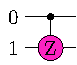
\includegraphics[height=0.1\textwidth]{src/crz_0.pdf}\raisebox{0.6cm}{=}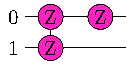
\includegraphics[height=0.1\textwidth]{src/alt_crz_1.pdf}\raisebox{0.6cm}{=}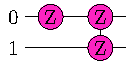
\includegraphics[height=0.1\textwidth]{src/alt2_crz_1.pdf}.
% \end{align}

\begin{equation}
    \tikzset{
        roundmini/.style={draw, circle, fill=unia2, text=white, inner sep=0.1pt, minimum size=1.2em, font=\small}
    }
    \begin{quantikz}
        \lstick{} & \ctrl{1} & \qw \\
        \lstick{} & \gate[style=roundmini]{\textcolor{white}{Z}} & \qw 
    \end{quantikz}
    =
    \begin{quantikz}
        \lstick{} & \gate[style=roundmini]{\textcolor{white}{Z}} \vqw{1} & \gate[style=roundmini]{\textcolor{white}{Z}} & \qw \\
        \lstick{} & \gate[style=roundmini]{\textcolor{white}{Z}}         & \qw                       & \qw 
    \end{quantikz}
    =
    \begin{quantikz}
        \lstick{} & \gate[style=roundmini]{\textcolor{white}{Z}} & \gate[style=roundmini]{\textcolor{white}{Z}} \vqw{1} & \qw \\
        \lstick{} & \qw                       & \gate[style=roundmini]{\textcolor{white}{Z}}         & \qw 
    \end{quantikz}
\end{equation}
where we lose the information about the angle (going from $\theta$ to $\theta/2$).
We can move the individual $R_z$ on the first qubit freely through the $R_{ZZ}$ gate on both qubits, since the $Z$ generator commutes with the $Z\otimes Z$ generator.\\
If we now apply the Pauli compiling scheme from before to the $R_{ZZ}$ gate, we get
\begin{equation}
    \tikzset{
        roundmini/.style={draw, circle, fill=unia2, text=white, inner sep=0.1pt, minimum size=1.2em, font=\small}
    }
    \begin{quantikz}
        \lstick{} & \gate[style=roundmini]{\textcolor{white}{Z}} & \gate[style=roundmini]{\textcolor{white}{Z}} \vqw{1} & \qw \\
        \lstick{} & \qw                       & \gate[style=roundmini]{\textcolor{white}{Z}}         & \qw 
    \end{quantikz}
= 
    \begin{quantikz}
        \lstick{} & \gate[style=roundmini]{\textcolor{white}{Z}} & \ctrl{1} & \qw & \ctrl{1} & \qw \\
        \lstick{} & \qw                       & \targ{} & \gate[style=roundmini]{\textcolor{white}{Z}}  & \targ{}         & \qw 
    \end{quantikz}
\end{equation}
% \begin{align}
% 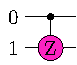
\includegraphics[height=0.1\textwidth]{src/crz_0.pdf}\raisebox{0.6cm}{=}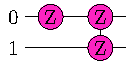
\includegraphics[height=0.1\textwidth]{src/alt2_crz_1.pdf}\raisebox{0.6cm}{=}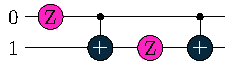
\includegraphics[height=0.1\textwidth]{src/alt3_crz_1.pdf}.
% \end{align}
Note that the $R_z$ on the first qubit can again be placed anywhere (since it's generator $Z$  commutes with the ``generator'' $\ket{1}\bra{1} = 1/2(1-Z)$ of the control in the \texttt{cnot}), so we have found a quite effective decomposition
\begin{equation}
    \tikzset{
        roundmini/.style={draw, circle, fill=unia2, text=white, inner sep=0.1pt, minimum size=1.2em, font=\small}
    }
    \begin{quantikz}
        \lstick{} & \ctrl{1} & \qw \\
        \lstick{} & \gate[style=roundmini]{\textcolor{white}{Z}} & \qw 
    \end{quantikz}
    =
= 
    \begin{quantikz}
        \lstick{} &  \ctrl{1} & \gate[style=roundmini]{\textcolor{white}{Z}} & \ctrl{1} & \qw \\
        \lstick{} &                       \targ{} & \gate[style=roundmini]{\textcolor{white}{Z}}  & \targ{}         & \qw 
    \end{quantikz}
\end{equation}
% \begin{align}
% 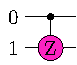
\includegraphics[height=0.1\textwidth]{src/crz_0.pdf}\raisebox{0.6cm}{=}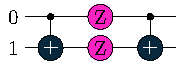
\includegraphics[height=0.1\textwidth]{src/alt4_crz_1.pdf}.
% \end{align}
Note that if the original angle was $CR_z(\theta)$, then the two parametrized gates are $R_z(\theta/2)$ (for the gate on the first qubits) and $R_z(-\theta/2)$ (for the gate on the second) -- so two different angles, not visible in the graphical representation.\\

What works with a single control also works with multiple control qubits.
\begin{algo*}[Multi-Control-Compilation] Take an $N$-qubit unitary
\begin{align}
    U = e^{-i\frac{\theta}{2} G}
\end{align}
acting on qubits $\left\{t_1,t_2,\dots,t_N\right\}$, then the controlled version with $M$ control qubits $\left\{c_1,c_2,\dots c_M\right\}$, is generated by 
\begin{align}
    \mathcal{G} = \prod_{k=1}^{M}\frac{1}{2}\left( 1-Z(q_k) \right) G(t_1,t_2,\dots,t_N).
\end{align}
\end{algo*}
As an example we take the Toffoli gate (the \textsc{ccnot}) and show the decomposition in graphical form.
We start with the generator for \textsc{not} which is $G=(X-1)$ and the gate itself is $X=e^{-i\frac{\pi}{2}(X-1)}$. The generator for Toffoli is therefore $-\frac{1}{4}\left(1-Z\right)\otimes\left(1-Z\right)\otimes\left(1-X\right) = -\frac{1}{4}\left(1-Z(1)-Z(2)-X(3)+Z(1)X(3)+Z(2)X(3)+Z(1)Z(2)-Z(1)Z(2)X(3)\right)$. Using a Hadamard operation on qubit 3 we diagonalize the $X(3)$ part of the generator and end up with
\[\frac{1}{4}\left(-1+Z(1)+Z(2)+Z(3)-Z(1)Z(3)-Z(2)Z(3)-Z(1)Z(2)+Z(1)Z(2)Z(3)\right).\] 
In the compilation of the gate we can then neglect the globale phase $e^{i\frac{\pi}{2}\frac{1}{4}}$ generated by the $1$ part of the generator~\footnote{note that you can only neglect the global phase in the final compilation, you can not neglect it, if you for example are building a controlled-Toffoli -- same as we could not neglect it here for the not gate.} and end up with a circuit of Pauli gates
\begin{equation}
    \tikzset{
        roundmini/.style={draw, circle, fill=white, text=white, inner sep=0.1pt, font=\small},
        squaremini/.style={draw, fill=white, text=white, inner sep=0.1pt, font=\small}
    }
    \begin{quantikz}
        \lstick{} & \ctrl{1} & \qw \\
        \lstick{} & \ctrl{1} & \qw \\
        \lstick{} & \targ{} & \qw 
    \end{quantikz}
    =
    \begin{quantikz}
        \lstick{} & \qw & \gate[style=roundmini]{Z} & \gate[style=roundmini]{Z} \vqw{1} & \gate[style=roundmini]{Z} \vqw{1} & \gate[style=roundmini]{Z} \vqw{2} & \qw & \qw & \qw \\
        \lstick{} & \qw & \gate[style=roundmini]{Z} & \gate[style=roundmini]{Z}         & \gate[style=roundmini]{Z}         & \qw                               & \gate[style=roundmini]{Z} \vqw{1} & \qw & \qw \\
        \lstick{} & \gate[style=squaremini]{H} & \gate[style=roundmini]{Z} & \qw & \gate[style=roundmini]{Z} & \gate[style=roundmini]{Z} & \gate[style=roundmini]{Z} & \gate[style=squaremini]{H} & \qw
    \end{quantikz}
\end{equation}
% \begin{align}
% 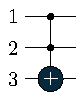
\includegraphics[height=0.15\textwidth]{src/toffoli.pdf}
% &\raisebox{1cm}{\;=\;}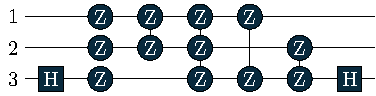
\includegraphics[height=0.15\textwidth]{src/toffoli_trotter.pdf} \nonumber\\
% \end{align}
which we can further decompose by the Pauli gate compiling scheme
% \begin{align*}
% \raisebox{1cm}{\;=\;}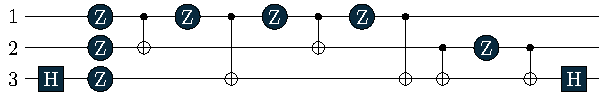
\includegraphics[height=0.1\textwidth]{src/toffoli_trotter_3.pdf} \nonumber\\
% \end{align*}
\begin{equation}
    \tikzset{
        roundmini/.style={draw, circle, fill=white, text=white, inner sep=0.1pt, font=\small},
        squaremini/.style={draw, fill=white, text=white, inner sep=0.1pt, font=\small},
    }
    \begin{quantikz}
        \lstick{1} & \qw & \gate[style=roundmini]{Z} & \ctrl{1} & \gate[style=roundmini]{Z} & \ctrl{2} & \gate[style=roundmini]{Z} & \ctrl{1} & \gate[style=roundmini]{Z} & \ctrl{2} & \qw      & \qw                       & \qw      & \qw \\
        \lstick{2} & \qw & \gate[style=roundmini]{Z} & \targ{}  & \qw                       & \qw      & \qw                       & \targ{}  & \qw                       & \qw      & \ctrl{1} & \gate[style=roundmini]{Z} & \ctrl{1} & \qw \\
        \lstick{3} & \gate[style=squaremini]{H} & \gate[style=roundmini]{Z} & \qw      & \qw                       & \targ{}  & \qw                       & \qw      & \qw                       & \targ{}  & \targ{}  & \qw                       & \targ{}  & \gate[style=squaremini]{H}
    \end{quantikz}
\end{equation}
and we have eliminated two pair of \textsc{cnot} gates on the way (as they are self inverse).


\subsection{Example: Oracle Construction (Part II)}
We will use the Pauli formalism to construct the quantum oracle used in the \texttt{Deutsch-Josza} algorithm
\begin{align*}
    U_f \ket{\mathbf{x}} = (-1)^{f(\mathbf{x})}\ket{\mathbf{x}}
\end{align*}
defined for standard basis states $\ket{\mathbf{x}}$ on $N$ qubits. 
We first note that we can also write 
\begin{align*}
    U_f \ket{\mathbf{x}} = e^{-\pi f(\mathbf{x})}\ket{\mathbf{x}},
\end{align*}
which opens up the path for generator based construction.
\begin{enumerate}
    \item Construct the Boolean function $f(\mathbf{x})$ as Hermitian generator $H\ket{\mathbf{x}}$
    \item Construct the Oracle as $U_f = e^{-i\pi H}$
\end{enumerate}
\subsubsection*{Construction of the generator}
We will use a Boolean formula in conjunctive normal form. Here, the formula consists of $M$ clauses $C_k$ connected through conjuctions (``and'' operations). Each clause contains literals (variables or negated variables) $u_i$ connected by disjunctions (``or'' operations). 
\begin{align*}
    f(\mathbf{x}) = \bigwedge_{k=1}^{M} \bigvee_{u\in C_k} u
\end{align*}
typical variants are $3$-SAT (each clause only has 3 literals at most) that look for example like
\begin{align*}
    f(\mathbf{x}) = \left(x_1 \vee x_2 \vee x_3\right) \wedge \left(\bar{x}_1 \vee x_4 \vee \bar{x}_8\right) \wedge \dots .
\end{align*}
Take for example a formula with 3 variables consisting of a single clause with 3 literals
\begin{align*}
    f(x_1,x_2,x_3) = x_1 \vee \bar{x}_2 \vee x_3
\end{align*}
the formula is always true, except for the assignment $x_1=0, x_2=1, x_3=0$. The generator 
\begin{align}
    H &= \ket{010}\bra{010} = \frac{1}{2^3}\left(1+Z(1)\right)\left(1-Z(2)\right)\left(1+Z(3)\right)\nonumber\\
    &= \frac{1}{8}\left(1+Z_1-Z_2+Z_3-Z_1Z_2+Z_1Z_3 - Z_2Z_3 - Z_1Z_2Z_3\right).
\end{align}
This generator has the same behaviour: eigenvalue 0 for basis state $\ket{010}$ and eigenvalue $+1$ for all other basis states.
In general the rule to construct a generator from a single clause is can be set to
\begin{align}
    \bigvee_{u\in C}^{} u \rightarrow H_C = \bigotimes_{k=1}^N p_k
\end{align}
with 
\begin{align}
    p_k = \begin{cases}
        \ket{0}\bra{0}, & x_k \in C\\
        \ket{1}\bra{1}, & \bar{x}_k \in C\\
        1, & \text{else}
    \end{cases}
\end{align}
where $x_k\in C$ is true, if the variable $x_i$ appears as literal in the clause. Note that we assume that trivial cases like $(x_k \in C) \wedge (\bar{x}_k\in C)$ have been removed from the clause.
For a general formula in conjunctive normal form, we can now construct a generator for each clause and multiply them together 
\begin{align*}
    f(\mathbf{x}) = \bigwedge_{k=1}^{M} \bigvee_{u\in C_k} u \rightarrow H_f = \prod_{k=1}^{M} H_{C_M}.
\end{align*}
This works, because our operator is diagonal (and therefore consists only of $1$ and $Z$ operations -- the products stay Hermitian (note that this is not in general the case).
\subsubsection*{Constructing the Oracle}
To construct the oracle as $U_f = e^{-\pi H_f}$ we don't need a Trotter decomposition (the generator is diagonal) and also no basis change (same reason). 
We will use the same example as in the previous chapter and just use the simple formula
\begin{align}
    f(\mathbf{x}) = (x_1\vee x_2\vee \bar{x}_3).
\end{align}
The generator is
\begin{align}
    H_f = \frac{1}{8}\left(1 + Z_1 + Z_2 - Z_3 + Z_1Z_2 + Z_1Z_3 - Z_2Z_3 - Z_1Z_2Z_3\right)
\end{align}
and the corresponding circuit is 
\begin{center} 
\tikzset{
        roundmini/.style={draw, circle, fill=unia2, inner sep=0pt, font=\small}
    }
\resizebox{\textwidth}{!}{%
\begin{quantikz}[column sep=0.7em, row sep=0.7em]
\lstick{$\ket{x_1}$} & \gate[style=roundmini]{\textcolor{white}{z}}       & \ctrl{1} & \qw  & \ctrl{1} & \ctrl{2} & \qw  & \ctrl{2} & \qw      & \qw  & \qw      & \ctrl{1} & \qw      & \qw  & \qw      & \ctrl{1} & \qw \\
\lstick{$\ket{x_2}$} & \gate[style=roundmini]{\textcolor{white}{z}}       & \targ{}  & \gate[style=roundmini]{\textcolor{white}{z}}  & \targ{}  & \qw      & \qw  & \qw      & \ctrl{1} & \qw  & \ctrl{1} & \targ{}  & \ctrl{1} & \qw  & \ctrl{1} & \targ{}  & \qw \\
\lstick{$\ket{x_3}$} & \gate[style=roundmini]{\textcolor{white}{z}}      & \qw      & \qw  & \qw      & \targ{}  & \gate[style=roundmini]{\textcolor{white}{z}}  & \targ{}  & \targ{}  & \gate[style=roundmini]{\textcolor{white}{z}}  & \targ{}  & \qw      & \targ{}  & \gate[style=roundmini]{\textcolor{white}{z}}  & \targ{}  & \qw      & \qw
\end{quantikz}%
}
\end{center}

Compared to the old construction (lets call this the direct construction), this seems way simpler (but less straightforward on first glance).~\footnote{Exercise: The circuit currently reflexts the order by which the individual parts of the generator where denotes in the equation above. Since all parts commute the order does not matter here. By changing the order of the individual parts of the generator, you can save up to four \texttt{cnot} operations.} Notable differences
\begin{itemize}
    \item Direct construction needs auxiliary helper qubits
    \item Direct construction results in a deeper circuit~\footnote{the decomposition of the triple and double controlled nots will take its toll}
    \item Direct construction does not need parametrized gates, like the $R_z(\pm \pi/4)$ gates used here but uses only classical logic gates (except for that two Hadamards). This can become a technical issue, when multiple clauses are involved and the angles become smaller and smaller through multiplication operations. 
\end{itemize}

To avoid the issue of exponentially vanishing angles, we could resort to a hybrid strategy: encode each clause with the Pauli formalism, saving in circuit depth by avoiding direct construction through multi-controlled not operations, but chosing the operation such that the result of a single clause is stored on one additional qubit. In the end we have at most as many additional qubits as clauses, these can then be checked with and gates (Toffoli operations). 
For this to work we would need an operation
\begin{align}
    U\left(\ket{0}\otimes\ket{\mathbf{x}}\right) =  \ket{C(\mathbf{x})}\otimes\ket{\mathbf{x}}
\end{align}
where a single qubit in the first register suffices, since for a single clause $C(\mathbf{x})\in \left\{0,1\right\}$.
The Quantum Phase Estimation (\texttt{QPE}) is an algorithm that does the job.


